\documentclass[14pt,a4paper]{extarticle}
\usepackage[utf8]{inputenc}

\usepackage[english,russian]{babel}
\usepackage{indentfirst}
\usepackage{amsmath}
\usepackage{amsfonts}
\usepackage{amssymb}
\usepackage{color}
\usepackage{float}
\usepackage{placeins}
\usepackage{mathrsfs}

\numberwithin{equation}{section}


\usepackage[version=3]{mhchem}% Package for chemical equation typesetting
%\renewcommand{\thefigure}{\thechapter.\Alph{figure}}


\usepackage{lineno}
%\linenumbers

\usepackage[usenames,dvipsnames,svgnames,table]{xcolor}
\usepackage[hypcap]{subcaption}
% \usepackage[colorlinks=true, linkcolor=Maroon, citecolor=ForestGreen]{hyperref}
\usepackage[colorlinks=false]{hyperref}
\usepackage{graphicx}
\usepackage{subcaption}
\usepackage[height=25cm, a4paper, hmargin={2.5cm, 1.5cm}, vmargin={2cm, 2.3cm}]{geometry}
\setlength{\parindent}{1em}
\setlength{\parskip}{0pt}% {.3em}

\usepackage{titlesec}
\titleformat*{\section}{\normalsize\bfseries}
\titleformat*{\subsection}{\normalsize\bfseries}
%\titlelabel{\thetitle.\quad}




\usepackage[separate-uncertainty = true, multi-part-units=single, range-phrase=--, range-units=single]{siunitx}

%\mathchardef\period=\mathcode`.
%\DeclareMathSymbol{.}{\mathord}{letters}{"3B}

\usepackage{setspace}
\onehalfspacing

\usepackage[backend=bibtex, style=numeric, sorting=none, maxnames=3, minnames=3, hyperref=true, url=true, isbn=false, backref=true]{biblatex}
\bibliography{mybib}

\usepackage{tocloft}
\usepackage{tikz}
\hyphenation{Ha-ma-ma-tsu}

%\newcommand{\RNum}[1]{\uppercase\expandafter{\romannumeral #1\relax}}

\usepackage{titletoc}
\dottedcontents{section}[3em]{}{2.9em}{1pc}
\dottedcontents{subsection}[3em]{}{2.3em}{1pc}
%\renewcommand{\thesection}{\thechapter\arabic{section}}
%\renewcommand{\thesection}{\thechapter\arabic{subsection}.}

\renewcommand{\figurename}{Рис.}
%\usepackage[labelsep=period, font=small]{caption}

\usepackage{titlesec}
\usepackage{physics}
\titlespacing*{\section}
{0pt}{1pt}{0pt}
% {0pt}{5.5ex plus 1ex minus .2ex}{4.3ex plus .2ex}
\titlespacing*{\subsection}
{0pt}{1pt}{0pt}
% {0pt}{5.5ex plus 1ex minus .2ex}{4.3ex plus .2ex}

\usepackage{fancyhdr}

\pagestyle{fancy}
\fancyhf{}
%\fancyhead[LE,RO]{Share\LaTeX}
%\fancyhead[RE,LO]{Guides and tutorials}
%\fancyfoot[CE,CO]{\leftmark}
\fancyfoot[LE,RO]{\thepage}
\renewcommand{\headrulewidth}{0pt}
\DeclareMathOperator{\sinc}{sinc}

\begin{document}
\section{Излучение релятивистской электрона в синусоидальном магнитном поле}
В этой части мы дадим вывод излучения релятивистского электрона в $r\omega$-пространстве, движущегося в синусоидальном магнитном поле. Единственно приближение, которым мы будем пользоваться, --- прааксиальное приближение. Вывод интересен тем, что даёт наглядное представление о спектре частицы, угловом распределении интенсивности в зависимости от резонансной частоты. В заключении главы, будет приведён вывод распределения электромагнитного поля(в ближней зоне???) через потенциалы Лиенара-Вихерта, будет получен результат, который даст представление о методах используемых в численных симуляциях, на примере кода SRW. В наших рассуждениях мы следовали (Салдин Гелони)
\subsection{Уравнение движения электрона в ондуляторе}
Выведем спектр излучения из ондулятора. Вывод начнём с уравнения движение релятивистского электрона в магнитном поле.

\begin{equation}
	\vec{F} = e[\vec{v} \times \vec{B}],
\end{equation} 
где $e$ --- заряд электрона, а $\vec{v}$ и $\vec{B}$ скорость частицы и магнитное поле соответственно. Уравнение можно переписать в виде:

\begin{equation}
	\cfrac{d\vec{p}}{dt} = \cfrac{e}{\gamma m_e}[\vec{v} \times \vec{B}],
\end{equation}
где $\gamma$ --- лоренц фактор, появившийся из релятивистского импульса. Направим ось $z$ вдоль направления релятивистского движения электрона и введём магнитное поле в ондуляторе $B_0\cos(k_w z)$, направленное вдоль оси $y$, где $k_w$ связана с периодом ондулятора следующим образом $k_w = 2\pi/\lambda_w$. 

\begin{equation}
	\label{eq:eq_of_motion}
	\begin{cases}
		\cfrac{d^2 x}{dt^2} = - \cfrac{e B_0}{\gamma m_e}\cfrac{dz}{dt} \cos(k_w z)\\
		\cfrac{d^2 z}{dt^2} = \cfrac{e B_0}{\gamma m_e}\cfrac{dx}{dt} \cos(k_w z)
	\end{cases} 
\end{equation}

один раз интегрируя первой уравнение из системы с заменой $dz = \beta cdt$, где $\beta = \|\vec{v}\| /c$, можно получить: 

\begin{equation}
 	\label{eq:dx/dt}
	\cfrac{dx}{dt} = - \cfrac{eB_0}{\gamma m_ek_w} \sin(k_w z)
\end{equation}
Введём коэффициент ондуляторности --- $K = \cfrac{eB_0 \lambda}{2\pi m_ek_w}$, который показывает угол отклонения электрона от оси $z$(?????). 

Подставляя получившийся результат~\ref{eq:dx/dt} во второе уравнение системы~\ref{eq:eq_of_motion} и интегрируя с пределами интегрирования от $0$ до некоторого $z_0$, получим систему:

\begin{equation}
	\begin{cases}
	\label{eq:eq_of_motion_velocity}
		\cfrac{dx}{dt} = - \cfrac{Kc}{\gamma} \sin(k_w z)\\
		\cfrac{dz}{dt} = \beta c - \cfrac{K^2 c}{2 \gamma^2 \beta}\sin^2(k_w z)
	\end{cases} 
\end{equation}

Проинтегрировав оба уравнения(в каких пределах?), получим (Wiedemann),

\begin{equation}
	\begin{cases}
	\label{eq:eq_of_motion_trej}
		x = \cfrac{Kc}{с\gamma k_w \beta} \cos(k_w\overline{\beta}ct)\\
		z = \overline{\beta}ct + \cfrac{K^2}{8 \beta^2 \gamma^2 k_w}\sin(2k_w\overline{\beta}ct), 
	\end{cases} 
\end{equation}
где был введено обозначение $\overline{\beta}$, которое определяется как $\overline{\beta}c = \beta c(1 - \cfrac{K^2}{4 \beta^2 \gamma^2})$
Из~\ref{eq:eq_of_motion_velocity} видно, что продольная скорость испытывает о осцилляции с удвоенной частотой...
\subsection{Решение волнового уравнения в прааксиальном приближении}
Вывод спектра излучения будем проводить в $r\omega$-пространстве. Начнём с уравнений Максвелла в вакууме:
\begin{equation}
	\begin{cases}
		\nabla \cdot \vec{E} = 4\pi \rho\\
		\nabla \cdot \vec{E} = 0\\
		[\nabla \times \vec{E}] = -\cfrac{1}{c} \cfrac{d\vec{B}}{dt}\\
		[\nabla \times \vec{B}] = \cfrac{4\pi}{c} \vec{j} + \cfrac{1}{c} \cfrac{\partial\vec{E}}{\partial t}
	\end{cases} 
\end{equation}
Из уравнений тривиально можно получить неоднородное волновое уравнение(какая калибровка?): 
\begin{equation}
	\label{eq:inhomo_wave_eq_xt}
	\pdv[2]{\vec{E}}{t} + c^2 \nabla^2 \vec{E} = 4\pi c^2 \nabla \rho + 4\pi \pdv{\vec{j}}{t}
\end{equation}
Это же уравнение перепишем в $r\omega$-пространстве, определив преобразование Фурье следующим образом:
\begin{equation}
	\label{eq:Fourier_wt}
	\begin{array}{lcl}
		\vec{\widetilde{E}}(r, \omega) = \displaystyle\int\limits_{-\infty}^{\infty} dt \vec{E}(r, t)\exp[-i\omega t]\\
		\\
		\vec{E}(r, \omega) = \cfrac{1}{2\pi}\displaystyle\int\limits_{-\infty}^{\infty} d\omega \vec{\widetilde{E}}(r, t)\exp[i\omega t]
	\end{array}
\end{equation}
Применив к уравнению~\ref{eq:inhomo_wave_eq_xt}, получим:
\begin{equation}
	\omega^2 \vec{\widetilde{E}} + c^2 \nabla^2 \vec{\widetilde{E}} = 4\pi c^2 \nabla  \widetilde{\rho} - 4i\pi\omega\vec{\widetilde{j}}
\end{equation}
Перепишем это уравнение в приближении медленно меняющейся амплитуды в сравнение с частотой осцилляций, что есть $\vec{\widetilde{E}} =  \vec{\overline{E}}\exp[i\omega z/c]$, в приближении $\cfrac{\partial |E|}{\partial z} \ll \cfrac{\omega}{c}|E|$. Где временная зависимость разложена до нулевого порядка малости, исходя из уравнения~\ref{eq:eq_of_motion_trej}. Получим:
\begin{equation}
	\label{eq:wave_slow_vary}
	c^2\bigg(\nabla^2 \vec{\widetilde{E}} - \cfrac{2i\omega}{c}\pdv{\vec{\widetilde{E}}}{z}\bigg)\exp[i\omega z/c] = 4\pi c^2 \nabla  \widetilde{\rho} - 4i\pi\omega\vec{\widetilde{j}}
\end{equation}

Для электрона движущегося в вакууме ток и плотность заряда выражается через дельта-функцию Дирака:

\begin{equation}
	\begin{array}{lcl}
		\rho(r,t) = -e\delta(\vec{r}- \vec{r'}(t)) = -\cfrac{e}{v_z(z)}\delta(\vec{r}_{\bot}- \vec{r'}_{\bot}(z))\delta(\cfrac{s(z)}{v} - t)\\
		\vec{j}(r,t) = \vec{v}\rho(r,t)	
	\end{array}
\end{equation} 
В $r\omega$-пространстве: 
\begin{equation}
	\begin{array}{lcl}
		\widetilde{\rho}(r,\omega) = -\cfrac{e}{v_z(z)}\delta(\vec{r}_{\bot}- \vec{r'}_{\bot}(z))\exp[\cfrac{iws(z)}{v}]\\
		\widetilde{\vec{j}}(r,\omega) = \vec{v}\widetilde{\rho}(r,\omega)	
	\end{array}
\end{equation} 
Подставим фурье-образы плотности тока и заряда в уравнение~\ref{eq:wave_slow_vary}, (где производная по градиентному члену? добавить это)
\begin{equation}
	\label{eq:wave_eq}
	\begin{array}{lcl}
		\nabla^2 \vec{\widetilde{E}} - \cfrac{2i\omega}{c}\cfrac{\partial\vec{\widetilde{E}}}{\partial z} = 
		\cfrac{4\pi e}{v_z(z)} \exp[iw\bigg(\cfrac{s(z)}{v} - \cfrac{z}{c}\bigg)]
		\bigg(  
			\cfrac{i\omega}{c^2}\vec{v}(z)
			-\nabla\bigg) \delta(\vec{r}_{\bot} - \vec{r'}_{\bot}(z)) 
		
	\end{array}
\end{equation} 
Получившиеся уравнение является точным. Теперь мы можешь применить параксиальное приближении. 
\begin{equation}
	\label{eq:wave_slow_vary_parax}
	\begin{array}{lcl}
		\nabla_{\bot}^2 \vec{\widetilde{E}}_{\bot} - \cfrac{2i\omega}{c}\cfrac{\partial\vec{\widetilde{E}}_{\bot}}{\partial z} = 
		\cfrac{4\pi e}{v_z(z)} \exp[iw\bigg(\cfrac{s(z)}{v} - \cfrac{z}{c}\bigg)]\bigg(  
			\cfrac{i\omega}{c^2}\vec{v}_{\bot}(z) 
			-\nabla_{\bot}\bigg) \delta(\vec{r}_{\bot} - \vec{r'}_{\bot}(z)) 
	\end{array}
\end{equation} 
Вторая производная по z, появляющаяся из оператора Лапласа полагается много меньшим по сравнению с первой производной по $z$ в уравнении~\ref{eq:wave_slow_vary_parax} исходя из предположения медленно меняющейся амплитуды.

Перед нами неоднородное дифференциальное уравнение в частных производных, которое решается с помощью функции Грина. Для дифференциального оператора $\partial_t - k\nabla_{2D}^2$ функция Грина есть: $\cfrac{1}{4\pi kt}\exp[-\rho^2/4kt]$. В частности для уравнения~\ref{eq:wave_slow_vary_parax}
\begin{equation}
	\label{eq:Green_func}
	G(z_0 - z'; \vec{r}_{\bot 0} - \vec{r'}_{\bot}) = 
	- \cfrac{1}{4\pi (z_0 - z')}\exp[i\omega \cfrac{|\vec{r}_{\bot 0} - \vec{r'}_{\bot}|^2}{2c(z_0 - z')}]
\end{equation} 
Получим решение для функции распределения поля:

\begin{equation}
	\begin{array}{lcl}
		\vec{\widetilde{E}}_{\bot}(z_0,  \vec{r}_{\bot 0}, \omega) = -\cfrac{e}{c}  \displaystyle\int\limits_{-\infty}^{\infty}\int\limits_{-\infty}^{\infty} dz'd\vec{r'}\cfrac{1}{z_0 - z'}
		\bigg(\cfrac{i\omega}{c^2}\vec{v}_{\bot}(z')
		-\nabla'_{\bot}\bigg) \delta(\vec{r'}_{\bot} - \vec{r'}_{\bot}(z'))\times\\
		\exp[iw\bigg( \cfrac{|\vec{r}_{\bot 0} - \vec{r'}_{\bot}|^2}{2c(z_0 - z')} +\cfrac{s(z')}{v} - \cfrac{z'}{c} \bigg)]
	\end{array}	
\end{equation}
Проинтегрировав по $d\vec{r'}$ получим общее решение уравнения~\ref{eq:wave_eq} :
\begin{equation}
	\label{eq:field_in_parax}
	\begin{array}{lcl}
		\vec{\widetilde{E}}_{\bot}(z_0,  \vec{r}_{\bot 0}, \omega) = -\cfrac{i\omega e}{c^2}  \displaystyle\int\limits_{-\infty}^{\infty} dz'
		\cfrac{1}{z_0 - z'}
		\bigg(\cfrac{\vec{v}_{\bot}(z')}{c}
		- \cfrac{\vec{r}_{\bot 0} - \vec{r'}_{\bot}(z')}{(z_0 - z')}\bigg)\times\\
		\exp[iw\bigg(\cfrac{|\vec{r}_{\bot 0} - \vec{r'}_{\bot}(z')|^2}{2c(z_0 - z')} + \cfrac{s(z')}{v} - \cfrac{z'}{c} \bigg)]
	\end{array}	
\end{equation}
Что есть распределение электромагнитного поля в точке наблюдения $\vec{r}_0$.

\subsection{Излучение планарного ондулятора}
В этой секции мы рассмотрим излучение планарного ондулятора использую наши предыдущие результаты~\ref{eq:field_in_parax} и~\ref{eq:eq_of_motion_trej}. Сперва проанализируем получившиеся распределение поля~\ref{eq:field_in_parax}: в случае ондулятора, член $(z_0 - z')^{-1}$ можно разложить около точки $z'$, так как размер ондулятора много меньше чем расстояние, с которого мы наблюдаем излучение: $\lambda_w N \ll z_0$, где $N$ число периодов ондулятора.

Воспользовавшись решениями~\ref{eq:eq_of_motion_velocity} и~\ref{eq:eq_of_motion_trej} и помня $\vec{r}_{\bot 0}/z_0 = \vec{\theta}$ преобразуем уравнение~\ref{eq:field_in_parax} к виду:
\begin{equation}
	\label{eq:field_in_parax}
	\begin{array}{lcl}
		\vec{\widetilde{E}}_{\bot}(z_0,  \vec{r}_{\bot 0}, \omega) =
		\cfrac{i\omega e}{c^2z_0} \exp[i\cfrac{\omega \theta^2 z_0}{2c}]
	 	\displaystyle\int\limits_{-\lambda_w N/2}^{\lambda_w N/2} dz'\exp[i\Phi_T]
		\bigg(\cfrac{K}{\gamma}\sin(k_w z)\vec{e_x} + \vec{\theta}\bigg)
	\end{array}	
\end{equation}
Здесь мы отбросили члены первого и большего порядка малости по $1/z_0$. Где за $\Phi_T$ мы обозначили:
\begin{equation}
	\Phi_T = 
	\bigg(\cfrac{\omega}{2c\widetilde{\gamma}^2} + 
	\cfrac{\omega\vec{\theta}^2}{2c}\bigg)z' - 
	\cfrac{K^2}{8\gamma^2}\cfrac{\omega}{k_w c}\sin(2k_wz') - \cfrac{K{\theta_x}}{\gamma}\cfrac{\omega}{k_w c}\cos(k_w z'),
\end{equation}
где $\widetilde{\gamma} = \cfrac{\gamma}{\sqrt{1 + K^2/2}}$.

Пределы интегрирования ограничили по длиной ондулятора от $-\lambda_w N/2$ до $\lambda_w N/2$, считая вклад в излучение от ондулятора доминирующим надо остальными вкладами от соответствующих участков траектории. На это шаге уже можно заметить, что излучение на оси будет линейно поляризованно, это есть вклад члена с током, вклад же плотности заряда или градиентный член, даёт вариацию поляризации, при наблюдении под некоторым углом $\theta$ к оси.

Если переписать~\ref{eq:field_in_parax} в следующе виде:
\begin{equation}
		\label{eq:field_in_parax_Bessel}
		\begin{array}{lcl}
			\vec{\widetilde{E}}_{\bot}(z_0,  \vec{r}_{\bot 0}, \omega) =
			\cfrac{i\omega e}{c^2z_0} \exp[i\cfrac{\omega \theta^2 z_0}{2c}]
			\displaystyle\sum_{m,n=-\infty}^{+\infty}
			J_m\bigg(-\cfrac{K^2}{8\gamma^2}\cfrac{\omega}{k_w c}\bigg)
			J_n\bigg(-\cfrac{K{\theta_x}}{\gamma}\cfrac{\omega}{k_w c}\bigg)\times\\
			\exp[\cfrac{i\pi n}{2}]
			\displaystyle\int\limits_{-\lambda_w N/2}^{\lambda_w N/2} dz'\exp[i(2m + n)k_wz']
			\bigg(\cfrac{K}{2i\gamma}\big(\exp[2ik_w z'] - 1\big)\vec{e_x} + \vec{\theta}\exp[ik_w z']\bigg)\times\\
			\exp[i\bigg(k_w \cfrac{\Delta\omega}{\omega_r} + 
			\cfrac{\omega\vec{\theta}^2}{2c}\bigg)z'],
		\end{array}	
\end{equation}
Где мы ввели $\omega = \omega_r + \Delta\omega$, $\omega_r = 2c\widetilde{\gamma}^2k_w$ и использовали формулу Якоби — Ангера:
\begin{equation}
	\begin{array}{lcl}
		\exp[iz\cos(\theta)] = 
		\displaystyle\sum\limits_{n =-\infty}^{\infty}
		i^n J_n(z)\exp[in\theta]\\	
		\exp[iz\sin(\theta)] = 
		\displaystyle\sum\limits_{n =-\infty}^{\infty}
		J_n(z)\exp[in\theta]
	\end{array}	
\end{equation}




До сих пор мы пользовались только двумя приближениями, --- медленно меняющейся амплитудой и параксиальным приближением, теперь можем воспользоваться следующим параметром --- количеством периодов ондулятора, --- $N$. Для этого обратим внимание на первой слагаемое в фазовом множителя под интегралом, и заметим, что если $k_w \cfrac{\Delta\omega}{\omega_r} + 
\cfrac{\omega\vec{\theta}^2}{2c} \ll k_w$, то фаза меняется медленно на одном периоде и эта фаза не занулит интеграл. Отметим, что для резонанса условия должны выполняться по отдельности, т.е. $\cfrac{\Delta\omega}{\omega_r} \ll 1$ и $\cfrac{\omega\vec{\theta}^2}{2c} \ll 1$, последнее даёт углы наблюдения вблизи резонанса: $\theta^2 \ll \cfrac{1}{\widetilde{\gamma}^2}$. Теперь необходимо обратить внимание на аргументы функций Бесселя, а именно: 
\begin{equation}
	\begin{array}{lcl}
		u = -\cfrac{K^2}{8\gamma^2}\cfrac{\omega}{k_w c}\\
		v = -\cfrac{K{\theta_x}}{\gamma}\cfrac{\omega}{k_w c} = - \cfrac{K{\theta_x}}{\gamma}
		\bigg(1 + \cfrac{\Delta\omega}{\omega_r}\bigg)2\widetilde{\gamma}^2 \lesssim
		\cfrac{2K{\theta_x}\widetilde{\gamma}}{\sqrt{1 + K^2/2}} \lesssim \theta_x\widetilde{\gamma} \ll 1
	\end{array}	
\end{equation}
Зная, что $J_\alpha(x) \thicksim \displaystyle\sum\limits_{n =0}^{\infty} x^{2\beta + \alpha} $, видим, что вклад нулевого порядка по $\theta_x\widetilde{\gamma}$, т.е. $J_\alpha(x) \thicksim 1$ даёт только функция Бесселя с индексом $n = 0$. Здесь мы пока не учитываем градиентный член пропорциональный $\vec{\theta}$, таким образом из оставшихся фазовых множителей можно выписать условия на индекс $m$. Они определяются нулями в аргументах соответствующих фаз или $m = -1$ и $m = 0$, оба оставшихся члена пропорциональны $\cfrac{K}{\gamma}$. 

Теперь вернёмся к градиентному члену, вклад от которого занулиться при усреднении по длине ондулятора при $n = 0$, этот вклад даст ненулевой вклад при $n = 1 - 2m$, т.о. в ход пойдут следующие члены разложения $J_m(v)$. Однако, помня интересующий нас диапазон углов, члены разложения будут порядка $\theta_x v^m$, очевидно, что их вклады пренебрежимо малы по сравнению с вкладами токового члена $\vec{e}_x$. Учитывая выше сказанные приближения, перепишем~\ref{eq:field_in_parax_Bessel}
\begin{equation}
	\label{eq:field_dist_in_integral}
	\begin{array}{lcl}
		\vec{\widetilde{E}}_{\bot}(z_0,  \vec{r}_{\bot 0}, \omega) =
		\cfrac{\omega e}{2c^2z_0}\cfrac{K}{\gamma}\exp[i\cfrac{\omega \theta^2 z_0}{2c}]
		\bigg(J_1(v) - J_0(v)\bigg)\vec{e}_x\times\\
		\\
		\displaystyle\int\limits_{-\lambda_w N/2}^{\lambda_w N/2} dz'
		\exp[i\bigg(k_w \cfrac{\Delta\omega}{\omega_r} + 
		\cfrac{\omega\vec{\theta}^2}{2c}\bigg)z'],
	\end{array}	
\end{equation}
Интеграл легко берётся:
\begin{equation}
	\label{eq:field_dist_nonNorm}
	\begin{array}{lcl}
		\vec{\widetilde{E}}_{\bot}(z_0,  \vec{r}_{\bot 0}, \omega) =
		\cfrac{\omega eL}{c^2z_0}\cfrac{K}{\gamma}\exp[i\cfrac{\omega \theta^2 z_0}{2c}]
		\sinc[\bigg(k_w \cfrac{\Delta\omega}{\omega_r} + 
		\cfrac{\omega\vec{\theta}^2}{2c}\bigg)L/2]\vec{e}_x ,
	\end{array}	
\end{equation}
где введено обозначение: $A_{JJ} = J_1(v) - J_0(v)$. 

В следующем параграфе мы займёмся выводном влияния конченого эмиттанса на распределение излучения, чтобы облегчить выкладки мы введём нормализованные единицы.
\begin{equation}
	\label{eq:norm_units}
	\begin{array}{lcl}
		\hat{E}_{\bot} = \cfrac{c^2z_0\gamma \widetilde{E}_{\bot}}{e\omega KLA_{JJ}}\\
		\hat{\theta} = \theta\sqrt{\cfrac{\omega L}{c}}\\
		\hat{z} = \cfrac{z}{L} ,
	\end{array}	
\end{equation}
а также, 
\begin{equation}
	\hat{C} = CL = 2\pi N\cfrac{\Delta\omega}{\omega_r}
\end{equation}
Теперь уравнения~\ref{eq:field_dist_nonNorm} и~\ref{eq:field_dist_in_integral} могут быть переписаны в нормализованных единицах.
\begin{equation}
	\label{eq:field_dist_in_integral}
	\begin{array}{lcl}
		\hat{E}_{\bot} = e^{i\Phi}
		\displaystyle\int\limits_{-1/2}^{1/2} dz'
		\exp[i\bigg(\hat{C} + 
		\cfrac{\hat{\theta}^2}{2}\bigg)z'],
	\end{array}	
\end{equation}

\begin{equation}
	\label{eq:field_dist_Norm}
	\begin{array}{lcl}
		\hat{E}_{\bot} = e^{i\Phi}
		\sinc\bigg(\cfrac{\hat{C}}{2} + 
		\cfrac{\hat{\theta}^2}{4}\bigg),
	\end{array}	
\end{equation}
\begin{figure}
	\centering  
	\begin{minipage}{0.49\textwidth}
		\centering
		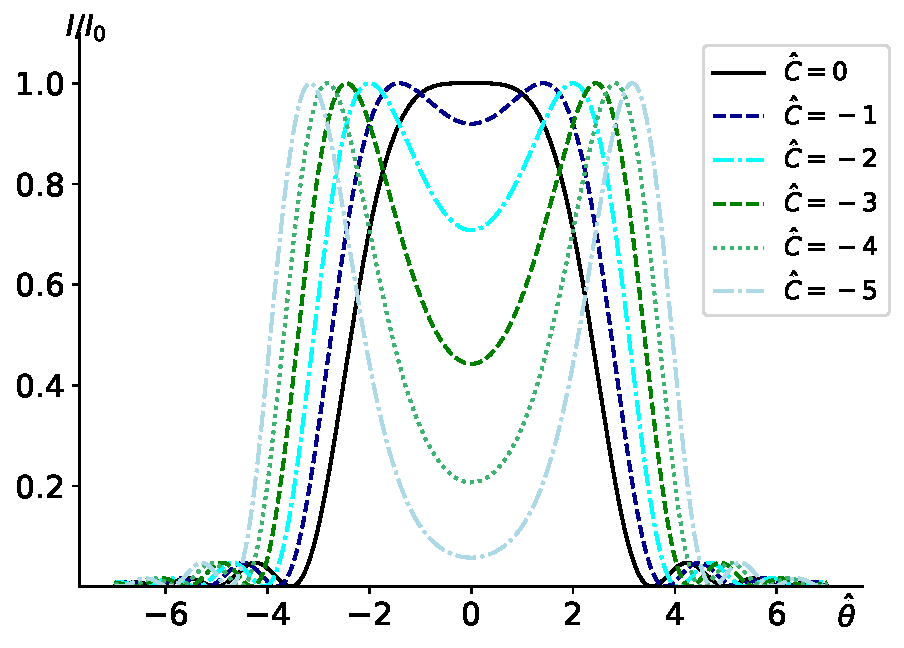
\includegraphics[width=\textwidth]{pic/angleC_neg.pdf}
		\caption{}
		\label{fig:angle_dist_C_neg}
	\end{minipage}\hfill
	\begin{minipage}{0.49\textwidth}
		\centering
		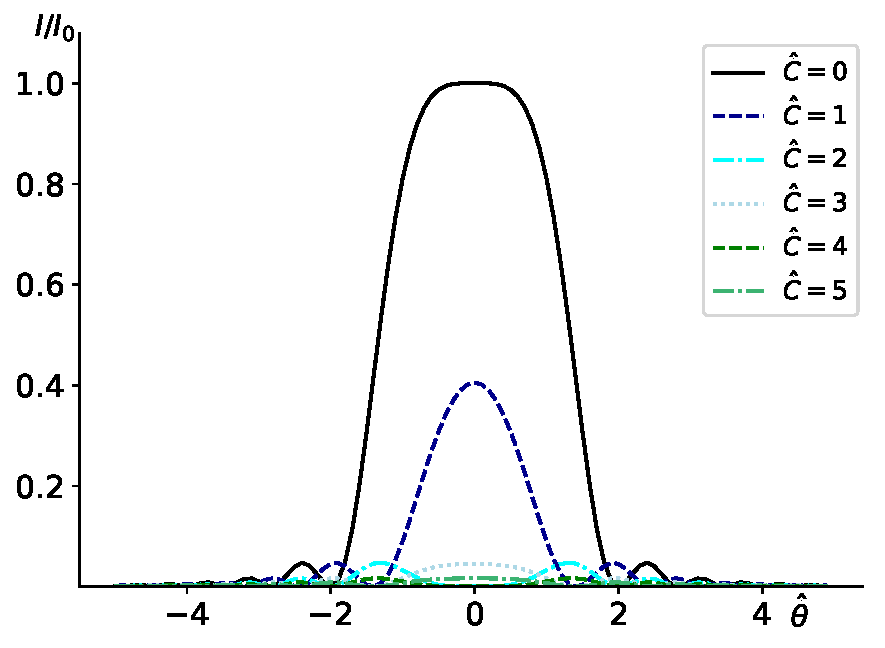
\includegraphics[width=\textwidth]{pic/angleC_pos.pdf}
		\caption{}
		\label{fig:angle_dist_C_pos}
	\end{minipage}    
\end{figure}
На рис.~\ref{fig:angle_dist_C_neg} и рис.~\ref{fig:angle_dist_C_pos} изображены угловые распределения излучения. Из них можно понять, что если сдвижка по спектру идёт в область меньших частот, то условие резонанса удовлетворяется на других углах и проинтегрированные по даст некоторую интенсивность. Если же сдвигаться по спектру в область более высоких частот, что условие резонанса на углах не будет выполняться и интенсивность быстро упадёт. На рис.~\ref{fig:spec_integrate_angle} представлен проинтегрированный по разным углам $\hat{\theta}$ спектр.
\begin{figure}[htbp]
	\centering
	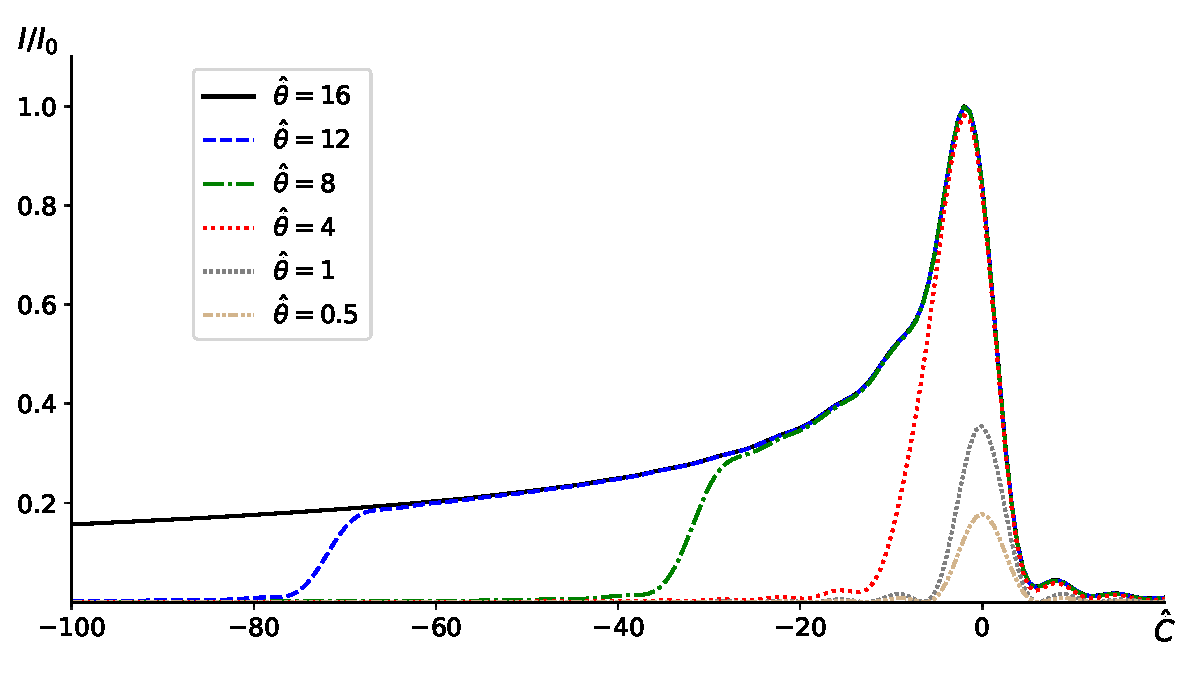
\includegraphics[width=.99\textwidth]{{pic/spec_integ_ang}.pdf}
	\caption{} 
	\label{fig:spec_integrate_angle}
\end{figure}
\subsection{Учёт конечности эмиттанса}
В этой параграфе мы покажем влияние эмиттанса пучка на спектр излучения и угловое распределение. Для начала перепишем уравнение~\ref{eq:field_dist_Norm} с учётом отклонения частиц от заданной траектории, --- $h_x$ и $h_y$ и с некоторым дополнительным углом $\eta_x$ и $\eta_x$. Сразу можно понять, что в уравнениие~\ref{eq:field_dist_Norm} можно сделать замену $\theta_{x,y} \rightarrow \theta_{x,y} - \eta_{x, y} - \cfrac{l_{x,y}}{z_0}$ и переписать углы в нормализованных единицах аналогично с~\ref{eq:norm_units}, с точностью до фазы: 
\begin{equation}
	\label{eq:field_dist_Norm}
	\begin{array}{lcl}
	\hat{E}_{\bot} \sim
	\sinc\bigg[\cfrac{\hat{C}}{2} + 
	\cfrac{1}{4}\bigg(\hat{\theta}_{x} - \hat{\eta}_{x} - \cfrac{l_{x}}{z_0}\bigg)^2 +
	\cfrac{1}{4}\bigg(\hat{\theta}_{y} - \hat{\eta}_{y} - \cfrac{l_{y}}{z_0}\bigg)^2\bigg],
	\end{array}	
\end{equation}
При этом можно положить  $\cfrac{l_{x,y}}{z_0} \ll 1$, что выполняется с очень высокой точностью. 

В наших рассуждениях мы будем использовать один предельный случай: электронный пучок не симметричен его вертикальны размер много меньше размера по радиальному направлению. Распределение частиц будем считать гауссовым: 
\begin{equation}
	\label{eq:field_dist_Norm}
	h_{x, y}(\eta_{x, y}) = \cfrac{N_e}{\sqrt{2\pi}\sigma_{x', y'}} \exp[-\cfrac{\eta^2_{x, y}}{2\sigma^2_{x', y'}}]
\end{equation}

Для удобства перепишем это распределение в нормализованных единицах, помня $\sigma_{x', y'} = \epsilon_{x', y'}/\beta_{x', y'}$, где $\epsilon_{x', y'}$ --- вертикальный и горизонтальный эмиттансы, $\beta_{0x', y'}$ --- минимум бета-функции, обычно минимум бета-функции выбирают в середине ондулятора. Нормализованные единицы для $\hat{\beta}_{0} = \beta_{0}$
и $\hat{\epsilon} = (\omega/c)\epsilon$
\begin{equation}
	\label{eq:field_dist_Norm}
	h(\hat{\eta}) = \cfrac{1}{\sqrt{2\pi\hat{\epsilon}/\hat{\beta}}} \exp[-\cfrac{\hat{\eta}^2\hat{\beta}_{0}}{2\hat{\epsilon}^2}]
\end{equation}
Как уже упоминалось мы будем рассматривать предельный случай $\epsilon_{y'}/\beta_{y'} \ll 1$, в то время как $\hat{\beta_0}_{x,y} \sim 1$, поэтому просто $\epsilon_{y'} \ll 1$. Теперь можно записать интенсивность поля следующий образом: 
\begin{equation}
	\label{eq:convolution}
	\hat{I} = \cfrac{1}{\sqrt{2\pi\hat{\epsilon}/\hat{\beta}}}
	\displaystyle\int\limits_{-\infty}^{\infty} d\hat{\eta}_x \sinc^2(\zeta)	
	\exp[-\cfrac{\hat{\eta}_x^2\hat{\beta}_{0x}}{2\hat{\epsilon}_x}],д
\end{equation}
Где мы ввели $\zeta = \cfrac{\hat{C}}{2} + 
\cfrac{1}{4}(\hat{\theta}_{x} - \hat{\eta}_{x})^2 +
\cfrac{1}{4}\hat{\theta}_{y}^2$.Здесь мы учли, что распределение по $y$ действует как дельта-функция. Предыдущее уравнение упрощается дальше в пределе $\hat{\epsilon}_x\hat{\beta}_x \gg 1$, опять же помня, что и $\hat{\beta}_x \sim 1$, получается $\hat{\epsilon}_x \gg 1$. Ширина $\sinc^2(\zeta)$ много больше ширины гауссвоского распределения, ширина которого $\hat{\epsilon}_x$, поэтому интеграл будет набираться в пике кардинального синуса и экспоненту можно вынести с аргументом: $\hat{\eta}_x = \hat{\theta}_x$: 
\begin{equation}
	\label{eq:convolution}
	\hat{I} = \cfrac{\exp[-\hat{\theta}_x^2\hat{\beta}_{0x}/2\hat{\epsilon}_x]}{\sqrt{2\pi\hat{\epsilon}/\hat{\beta}}}
	\displaystyle\int\limits_{-\infty}^{\infty} d\hat{\eta}_x \sinc^2\bigg(\cfrac{\hat{C}}{2} + 
	\cfrac{1}{4}(\hat{\theta}_{x} - \hat{\eta}_{x})^2 +
	\cfrac{1}{4}\hat{\theta}_{y}^2\bigg)	
\end{equation}
Этот интеграл можно взять числено. %введя очевидную замену $\hat{\eta_{x}} \rightarrow \hat{\theta}_x - \hat{\eta_{x}}$. 
На рис.~\ref{fig:spec} представлен спектр излучения одного электрона, на~\ref{fig:2spec_emittance_and_single} представлены: линия 1.: спектр излучения пучка с $\hat{\epsilon}_x\rightarrow \infty$  $\hat{\epsilon}_x\rightarrow 0$, линия 2.: одноэлектронный спектр как функция $\hat{C} + \hat{\theta}_y^2/2$ при $\hat{\theta}_x = 0$ 
\begin{figure}
	\centering  
	\begin{minipage}{0.49\textwidth}
		\centering
		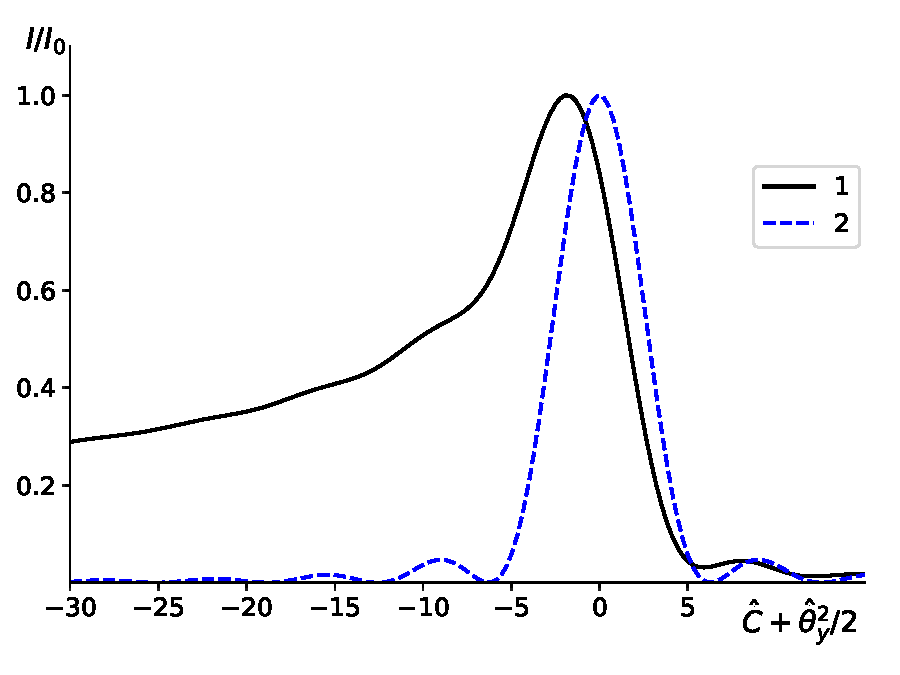
\includegraphics[width=\textwidth]{pic/spec_integ_emittance.pdf}
		\caption{}
		\label{fig:2spec_emittance_and_single}
	\end{minipage}\hfill
	\begin{minipage}{0.49\textwidth}
		\centering
		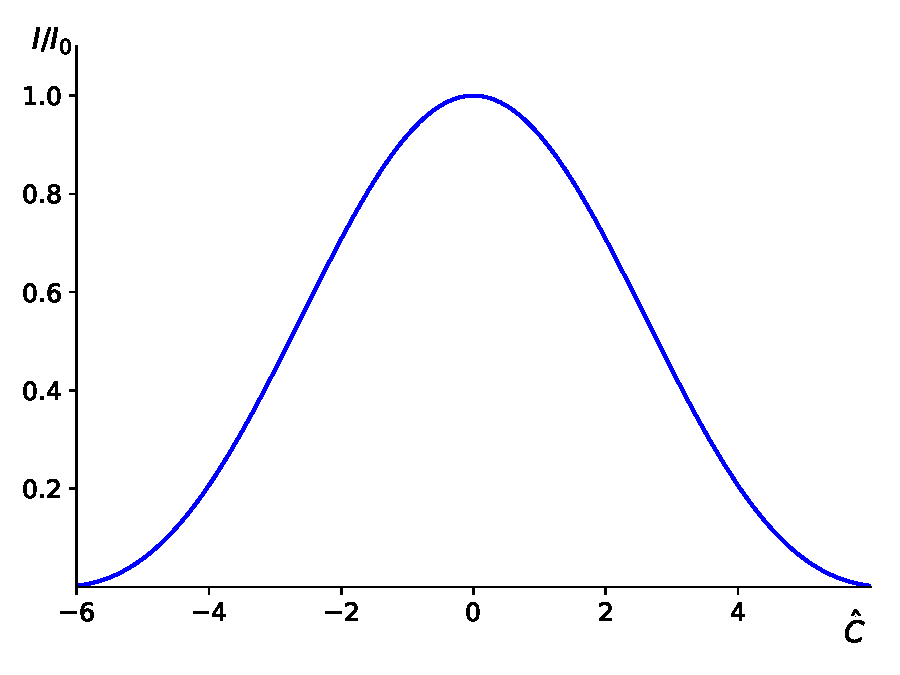
\includegraphics[width=\textwidth]{pic/spec_C.pdf}
		\caption{}
		\label{fig:spec}
	\end{minipage}    
\end{figure}
\section{Фурье оптика}
В этой главе мы предложим наглядный подход к решению задачи о распространение волнового фронта в пустом пространстве, его прохождении через систему линз и другие оптические элементы. Приведённые результаты напрямую могут быть использованы в программном коде. Распределение поля в начальный момент времени будем считать гауссовским, однако, как будет показано, развитый подход может быть использован для произвольного распределения поля. В наших выкладкам мы следуем подходу (Гудман, Салдин, Serkez)

\subsection{Распространение света в пустом пространстве}
Наши рассуждения мы начнём с волнового уравнения в пустом пространстве ($\vec{j} = 0, \rho = 0$). 
\begin{equation}
	\pdv[2]{\vec{E}}{t} + c^2 \nabla^2 \vec{E} = 0
\end{equation}

В  $r\omega$-пространстве уравнение приобретает знакомый вид уравнения Гельмгольца, где $k_0 = \omega/c$.

\begin{equation}
	k_0^2\vec{\widetilde{E}} + \nabla^2 \vec{\widetilde{E}} = 0
\end{equation}

Совершив фурье-преобразование в $k$-пространство по координатам $x,y$, которое определим схожим образом с~\ref{eq:Fourier_wt}:

\begin{equation}
	\label{eq:Fourier_rk}
		\begin{array}{lcl}
		\vec{\widehat{E}}(\vec{k}, \omega) = \displaystyle\int\limits_{-\infty}^{\infty}\int\limits_{-\infty}^{\infty} dxdy \vec{E}(\vec{r}, t)\exp[ik_xx + ik_xx]\\
		\\
		\vec{E}(\vec{r}, \omega) = \cfrac{1}{4\pi^2}\displaystyle\int\limits_{-\infty}^{\infty}\int\limits_{-\infty}^{\infty} dk_xdk_y \vec{\widehat{E}}(\vec{k}, t)\exp[-ik_xx - ik_xx],
	\end{array}
\end{equation}

получим: 
\begin{equation}
	k_0^2\Big(1 - \cfrac{k^2_x}{k^2_0} - \cfrac{k^2_y}{k^2_0} \Big)\vec{\widehat{E}} + \dv[2]{\vec{\widehat{E}}}{z} = 0
\end{equation}

Теперь можно напрямую можно получить решение этого обыкновенного дифференциального уравнения:
\begin{equation}
	\vec{\widehat{E}}(\omega, k_x, k_y, z) = \vec{\widehat{E}}(\omega, k_x, k_y, 0)\exp[ik_0z\sqrt{1 - \frac{k^2_x}{k^2_0} - \frac{k^2_y}{k^2_0}} ]
\end{equation}

Введём функцию отклика среды:

\begin{equation}
	H(k_x, k_y, z) = \cfrac{\vec{\widehat{E}}(\omega, k_x, k_y, z)}{\vec{\widehat{E}}(\omega, k_x, k_y, 0)} = \exp[ik_0z\sqrt{1 - \frac{k^2_x}{k^2_0} - \frac{k^2_y}{k^2_0}} ]
\end{equation}
 
Видно, чтобы получить распределение электромагнитного поля на некотором расстоянии $z$, необходимо совершить обратное преобразование Фурье в $xy$-пространство. Таким образом решение волнового уравнения сводиться к трём относительно простым операциям: первое, --- перевод начального распределения в $k_xk_y$-пространство, далее домножение получившегося распределения на функцию отклика среды, в нашем случае пустое пространство, и последний шаг, --- обратное преобразование Фурье. 

\subsection{Действие тонкой линзы на волновой фронт}
Тонкая линза 
\end{document}
























